\section{Graphical Passwords - Usability vs. Security}

    Authentication with text-based passwords are a common approach, but it is well known that users often choose weaker passwords because of the limitations of recalling text-based passwords. Graphical passwords came as an alternative solution for overcoming the limitations of text-based passwords, and was inspired by researchers that showed that the graphical memory of humans is particularly well-suited to remember graphical information. 
    Like text-based passwords schemes, graphical password schemes are also a knowledge-based authentication scheme, e.g. ``something you know'' that are described in the background theory. Since it all started around 1999, there have been many suggestions for graphical password schemes. 

    \begin{wrapfigure}{l}{0.35\textwidth}
      \vspace{-20pt}
      \begin{center}
        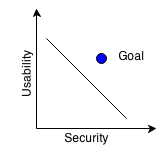
\includegraphics[scale=0.7]{pics/UsabilityVsSecurity.png}
      \end{center}
      \vspace{-20pt}
      \caption{Usability vs. Security}
      \vspace{-10pt}
    \end{wrapfigure}

    The problem with graphical password schemes is that they often promise improved password memorability and thus usability, while at the same time improving the security \cite{Biddle}.Since the first graphical password schemes was proposed, it is not widely in use. One of the problems with graphical approaches are that they require more overhead in the authentication phase. Like text-based passwords the users can simply type their passwords, while many of the graphical passwords require to go through many steps, requiring the user to spend more time in the authentication phase. The graphical password schemes like Passface and grIDsure are some of the graphical password schemes with commercial interest, while on mobile devices graphical passwords are not widely adopted. There is a known problem with authentication on mobile devices because of the difficulty of typing on mobile keyboards, making authentication schemes using alternatives getting increased attention. Because of the difficulty of writing on mobile keyboards it highlights the importance of understanding the usability and security implications.

    \begin{wrapfigure}{r}{0.35\textwidth}
      \vspace{-20pt}
      \begin{center}
        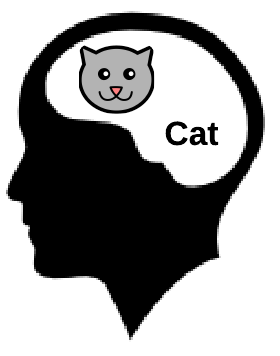
\includegraphics[scale=0.35]{pics/dualCoding.png}
      \end{center}
      \vspace{-20pt}
      \caption{Dual-Coding Theory}
      \vspace{-10pt}
    \end{wrapfigure}

    In many years, the field of psychology been a important in order to understand how humans interpret and remember different information. Psychology studies have recognized that the human brain have a superior memory for recognizing and recalling visual information rather recognizing and recalling verbal or textual information. One known theory is the ``dual-coding theory'', suggesting that verbal and non-verbal memory are processed and represented differently in humans mind. Text are verbal information that is represented symbolically, in contrast to non-verbal information like images that are mentally represented in a way that perceived concepts are assigned to a perceived meaning of what is directly observed. Both verbal and non-verbal information can be used when recalling information. For example, say a person have received stimulus of the concept ``cat'', both the image of a cat as well as the word ``cat''. When the person is asked to recall the concept ``cat'', the person can retrieve the image or the word individually, or both simultaneously. 
    If the word ``cat'' is recalled, the image of the cat is not lost and can still be retrieved at a later point in time. The ability to code a stimulus in two different ways can increase humans ability to remember, in contrast to only code the stimulus in one way.
    In the background theory there are described three different categories of graphical passwords according to the memory task involved in remembering and entering the password, e.g. recall, recognition and cued-recall. 

    In terms of authentication, its primary goal is to provide security for its intended environment in order to avoid security attacks. In knowledge-based authentication, e.g. ``something you know'', we classify attacks into two general categories: guessing and capturing attacks. In a guessing attack the attackers are able to search through the entire password space, or either predict the users passwords patterns in order to avoid searching through the whole passwords space (often referred to as a dictionary attack). When talking about capturing attacks, the attackers are directly obtain the passwords by observing the authentication process. One of the known capturing attacks on graphical passwords are shoulder surfing because of its graphical visualization.  


% ----------- Empirical vs. Practival password space --------%

    \begin{wrapfigure}{l}{0.4\textwidth}
      \vspace{-20pt}
      \begin{center}
        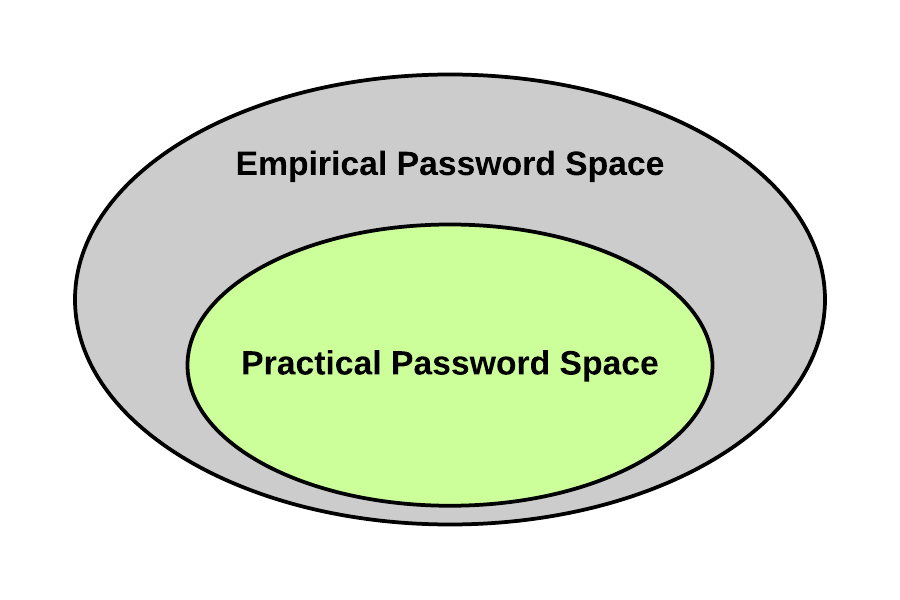
\includegraphics[scale=0.16]{pics/EmpiricalVsPractical.png}
      \end{center}
      \vspace{-20pt}
      \caption{Empirical vs. Practical Password Space}
      \vspace{0pt}
    \end{wrapfigure}

    When a user are able to make their own password, the password that is created is often influenced by different biases. A bias can be explained as a prejudice in favor of or against one thing, person, or group compared with another, usually in a way that influence a person choice of action. When we are talking about a bias in terms of passwords, a the password making process can be influenced by biases like the demography of a person or the visualization of the password scheme. Since a person needs to remember a password, it is normally to choose a password that are connected to you in order to remember the password, causing the password to have bias. The problem with many password schemes is that there are an empirical password space, but it seems that it is not the case in practice because of the biases that are often introduced, making the practical password space less than the empirical password space. In a case study of 14.000 Unix passwords, a research group found a 25\% of the passwords were in a group of words forming a dictionary of $3\times10^{6}$ words \cite{UnixPasswords}. This dictionary shows that an attacker can have a relatively high success rate with an attack, despite the fact that there a roughly $2\times10^{14}$ 8-character passwords consisting of digits, and upper case and lower case letters. Due to the limitations of human memory, useres often choose passwords which are easier to remember, causing a significant number of user-chosen password to fall into a small dictionary, e.g. practical password space \cite{Tao}. A well-designed dictionary is a tiny subset of the full password spave, e.g. theoretical password space, which further can be prioritized  according to the likelihood for a password to be chosen. It is therefore a commonly stated that the security of a password scheme is releted closely to the size of its memorable/practical password space, rather than its theoretical password space. Since psychological studies have recognized that the human brain have a superior memory for recognizing and recalling visual information, it support the statement that users are able to remember more complex graphical password form a larger password space than a alphanumeric password. Logically the attacker then have to build a bigger and more complex dictionary, thus spend more time to achieve the same success rate as for textual passwords. % Her må jeg ha noen eksempler på dictionary attacks mot grafiske passord!!!

% -----------------------------------------------


% ----------Research on Memorability --------%

    Write something about research on memorability

% --------------------------------------------%

    As stated earlier, the mobile phone have emerged as a good platform for graphical passwords because it is easier to input on touchscreen as a contrast to text-based passwords. Graphical passwords on mobile devices seems as a natural fit, as they often require direct manipulation of visual elements. 